\documentclass[12pt,oneside,openany,a4paper,%..... Layout
               afrikaans, english,%.............. Global language selection
               ]{memoir}
               
               
\usepackage{graphics}
\usepackage{epstopdf}
\usepackage{amsmath,bm}
\usepackage{tikz}
\usepackage{tikz-dimline}
\usepackage{tikz-timing}[]
\usepackage[siunitx]{circuitikz}
\usetikzlibrary{circuits.logic.US} % TiKZ Library for US Logic Circuits.
\usetikzlibrary{calc,arrows,shapes,shadows,matrix,positioning}
\usepackage{siunitx}
\usepackage[final]{pdfpages}
\usepackage[latin1]{inputenc}
\usepackage{standalone}
 \usepackage[masters-t,%.......................... Master thesis
             goldenblock,%........................ A5 type block (or a5block or wide)
            ]{usthesis}%.......................... US thesis style with memoir

%
% PLEASE read the USthesis documentation for the class options
% and how to set line and paragraph spacing
%



%==== Language setup ================================================
 \usepackage[latin1]{inputenc}%................... Recognizes �, �, etc
 \usepackage{babel}%.............................. Language setup

%==== Math setup ====================================================
 \usepackage{amsmath,bm}%............................ Advanced math (before fonts)
 %\usepackage{amssymb}%............................ AMS Symbol fonts

%==== Font setup (default is Computer Modern) =======================
 \usepackage[T1]{fontenc}%........................ Type 1 fonts
 %\usepackage{fourier}
 \usepackage{textcomp}%........................... Additional text character
 \usepackage{bm}%................................. Bold math symbols (after fonts)

%==== Ref's, Bib's and Nomencl ======================================
 \usepackage{usnomencl}%.......................... List of symbols (in usthesis pack)
 \usepackage{usbib}%.............................. Bibliography    (in usthesis pack)
    \bibliographystyle{usmeg-a}
    \renewcommand\bibfont{\small}

    %% For usmeg-a, the bib is a list of references. If you
    %% are using usmeg-n comment out the following lines
    \addto{\captionsafrikaans}{\renewcommand{\bibname}{Lys van Verwysings}}
    \addto{\captionsenglish}{\renewcommand{\bibname}{List of References}}

%==== Graphics and Color ============================================
\usepackage{graphicx}%........................... Graphicx loaded in usthesis
\usepackage{color}%.............................. Color setup
\usepackage{eso-pic}%............................ Shipout commands for watermark
    \newcommand*{\WaterMark}[2][0.15\paperwidth]{%
        \AddToShipoutPicture*{\AtTextCenter{%
                \parbox[c]{0pt}{\makebox[0pt][c]{%
                    \includegraphics[width=#1]{#2}}}}}}

%==== Local Defs ====================================================
\makeatletter

%
% Please insert user defined commands here
% and NOT in the document itself!
%

\makeatother

%==== TITLE PAGE ====================================================
\title{\bfseries
       \AorE{%-- Afrikaans ------------------------------------------
             Die Terugvoer Beheerwet van 'n Robotiese Gimnas\\[1ex]
             \normalfont\small\itshape
             (``The Feedback Control of a Robotic Gymnast'')
            }{%-- English -------------------------------------------
             The Feedback Control of a Robotic Gymnast
            }}

\author{H.\ Kotz�}{Henry Kotz�}

\degree{\AorE{BIng (Megatronika)}{BEng (Mechatronics)}}
       {\AorE{Magister in Ingenieurswese (Meganiese)}
             {Master of Engineering (Mechanical)}}

\address{\AorE{%-- Afrikaans ----------------------------------------
        Departement Meganiese en Megatroniese Ingenieurswese,\\
        Universiteit van Stellenbosch,\\
        Privaatsak X1, Matieland 7602, Suid Afrika.%
             }{%-- English ------------------------------------------
        Department of Mechanical and Mechatronic Engineering,\\
        University of Stellenbosch,\\
        Private Bag X1, Matieland 7602, South Africa.
             }}

\faculty{\AorE{Fakulteit Ingenieurswese}%
              {Faculty of Engineering}}

\supervisor{Dr.\ J.A.A \ Engelbrecht }
\cosupervisor{}

\setdate{10}{2018}

%\SetSponsor{The financial assistance of the National Research Foundation (NRF)
%    towards this research is hereby acknowledged. Opinions expressed and
%    conclusions arrived at, are those of the author and are not necessarily to
%    be attributed to the NRF.}


%====================================================================
%     MAIN DOCUMENT
%====================================================================
\maxsecnumdepth{subsubsection}
\maxtocdepth{section}

\begin{document}

%==== Front matter ==================================================
 \frontmatter
 \WaterMark{UScrest-WM}
 %\TitlePage
 %\begin{comment}

 
 
 

\begin{titlingpage}
	
	{	\centering
		\vfill
		\textbf{\Huge
			Project File for \\
			The Feedback Control Of A\\ 
			\vskip0.5cm
			Robotic Gymnast}
		\vskip0.5cm
		\normalsize by \\
		\vskip0.5cm
		\Large Henry Kotz\'{e} 
		\vskip1cm
		\large Mechatronic Project 448 
		\vskip2cm
		\small Project file submitted in partial fulfilment of the requirements of
		the module Mechatronic Project 448 for the degree Baccalaureus in
		Engineering in the Department of Mechanical and Mechatronic
		Engineering at the University of Stellenbosch 
		\vskip2cm
		\large Study leader: Dr. J.A.A Engelbrecht\\
		\vskip2cm
			\large October 2018\\
	}    
	\vfill
	\begin{figure}[t!]
		
\includegraphics[width=8cm]{UScrest-top.eps}
		\centering
		\vskip0.5cm
	\end{figure}
	% also works with logo.pdf
	\vfill
	\vfill
	%{\centering {\large \today\par} }
\end{titlingpage}
%\end{comment}
 \DeclarationDate{2018/10/27}
 \DeclarationPage

 %\begin{abstract}[english]%===================================================
In this report a design method for the swinging and balancing  of the underactuated robotic gymnast was researched, simulated and tested on a physical model. The electronic, mechanical and software designs are discussed to show how the physical model was constructed, controllers implemented and data acquired.
\end{abstract}


\begin{abstract}[afrikaans]%=================================================
In die projek word die swaaiende en balanseering beheerwette vir 'n robotiese gimnas genavors, ontwerp en getoets op 'n fisiese model. Die eletroniese, meganiese en sagteware ontwerpe word bespreek om ten einde te wys hoe die fisiese model, beheerders en so voort geimplementeer en getoets is.
\end{abstract}


\chapter{Acknowledgements}%==================================================

I would like to express my sincere gratitude to the following people
and organisations.\\

Dr. Japie Engelbrecht for supervising the project throughout the year. He provided critical feedback on progress, guided me in the correct direction and was a voice of reason throughout the project.\\

The Electrical and Electronic Department for allowing the use of their equipment and facilities. They allowed me to work with confidence ensuring the facilities and equipment are maintained with no interruption to my work.\\

Mr$.$ Croukamp, Mr$.$ van Eenden and Mr$.$ Lecholo for assisting me with the mechanical and electronic designs. The atmosphere in the manufacturing labotorium was always welcoming.\\

The group of final year student working together in the 4th floor labs. You all made the experience more worthwhile and encouraged me through  difficult times. 




\chapter{Dedications}%=======================================================
 \vfill
 \begin{Afr}
 \begin{center}\itshape
    Hierdie verslag word opgedra aan my ouers wat my ondersteun het tydens die 4 jaar om die graad van ingenieurswese te ontvang en die Here vir sy genade. 
 \end{center}
 \end{Afr}
 \vfill
 \clearpage

%============================================================================
\endinput


 \tableofcontents
 \clearpage

 \setcounter{lofdepth}{2}
 %\listoffigures
 \clearpage     

 %\listoftables
 \clearpage

 %\chapter{Nomenclature}

\begin{Nomencl}
 \NomGroup{Constants}%-----------------------------------------------
   \item[$\mathrm{g} = $] $\mathrm{9.81\,m/s^2}$

 \NomGroup{Variables}%-----------------------------------------------
 	\item[$I$]         \UnitLine{Inertia                }{kg{\cdot}m^2}
 	\item[$m$]         \UnitLine{mass                }{kg}
 	\item[$l$]         \UnitLine{Lenght                }{m}
	\item[$L$]         \UnitLine{Lenght                }{m}
  	\item[$R$]			\UnitLine{Reaction Force}		{N}
  	\item[$T$]      	\UnitLine{Torque                    }{N{\cdot}m}
  	\item[$F$]      	\UnitLine{Force                    }{N}
   	\item[$x$]         	\UnitLine{Coordinate                }{m}
   	\item[$\ddot{x}$]  	\UnitLine{Acceleration              }{m/s^2}\\
   	\item[$\theta$]    	\UnitLine{Rotation angle            }{rad}
   	\item[$\phi$]    	\UnitLine{Rotation angle            }{rad}
   	\item[$\dot{\theta}$]    	\UnitLine{Angular velocity            }{rad/s}
   	\item[$\dot{\phi}$]    	\UnitLine{Angular velocity            }{rad/s}
   	\item[$\ddot{\theta}$]    	\UnitLine{Angular acceleration            }{rad/s^2}
   	\item[$\ddot{\phi}$]    	\UnitLine{Angular acceleration            }{rad/s^2}
   	\item[$\zeta$]     	\UnitLine{Damping Coefficient        }{1}
   	\item[$t$]      	\UnitLine{Time                    }{s}
   	\item[$\tau$]      	\UnitLine{Torque                    }{N{\cdot}m}
   	\item[$J$]      	\UnitLine{Polar second moment of area                    }{m^4}
   	
   	

 \NomGroup{Vectors}%-------------------------------------
   \item[$\vec{q}$] Angular position vector
   \item[$\vec{\dot{q}}$] Angular velocity vector
   \item[$\vec{\ddot{q}}$] Angular acceleration vector

 \NomGroup{Subscripts}%----------------------------------------------
   \item[$a$] 			Unactuated Pendulum
   \item[$b$]          	Actuated Pendulum
   \item[$1$]          	Unactuated Pendulum center of mass
   \item[$2$]          	Actuated Pendulum center of mass
\end{Nomencl}



\endinput


%==== Main document =================================================
\mainmatter
   \setsecnumdepth{subsubsection}
%   \numberwithin{equation}{section}
%   \numberwithin{figure}{chapter}
%   \numberwithin{table}{chapter}

\chapter{Introduction}
\label{chp:introduction}


%%%%%%%%%%%%%%%%%%%%%%%%%%%%%%%%%%%%%%%%%%%%%%%%%%%%%%%%%%%%%%%%%%%%%%%
\section{Problem Statement}

In this report a feedback control system for a robotic gymnast that is able to swing from the "hanging" position to the "handstand" position will be designed, implemented and verified. Feedback control loops must be designed that use the "legs" of the gymnast to swing the "body" of the gymnast from the "hanging" position to a "handstand" position and then balance the gymnast on top of the horizontal bar. A mathematical model for the dynamics of the swinging robotic gymnast system must be derived or sourced from literature. The dynamics are analysed to propose an appropriate feedback control architecture that actuates the "legs" of the gymnast using feedback from sensors that measure the swinging motion of the gymnast on a horizontal bar. A practical demonstrator must be constructed and the correct operation must be demonstrated.\\

\section{The Robotic Gymnast System}
\begin{figure}[h]
	\centering
	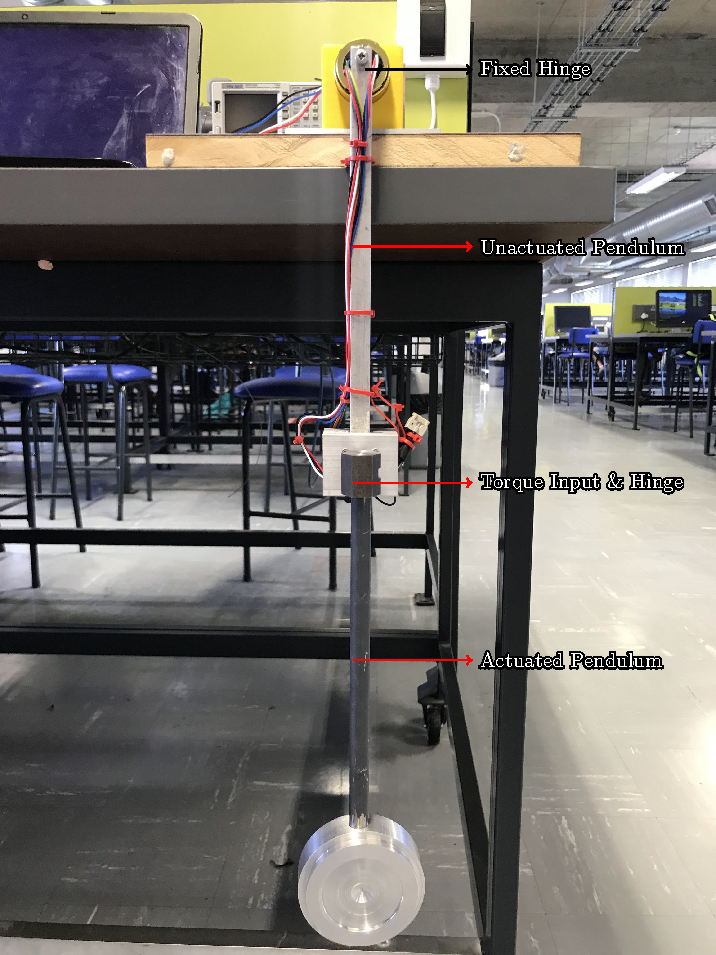
\includegraphics{./figs/overview/overview.pdf}
	\caption{Overview of the Robotic Gymnast System}
	\label{fig:overview}
\end{figure}

Figure \ref{fig:overview} provides an overview of the system to create a mental picture for the variables and concepts used throughout the report. There are 2 pendulums that are attach together with a hinge. At this hinge there is a torque being applied by a motor to the actuated pendulum. The entire system rotates around the fixed hinge at the top to which the unactuated pendulum is connected. The system is describe using two independent parameters, $\theta$ and $\phi$ which describes the entire system.\\

The goal is to use the feedback of the independent parameters to apply a torque to the actuated pendulum to swing the gymnast from the hanging position and balance in the inverted position. This is accomplished by designing a microcontroller to interface with sensors to provide information about the independent parameters and implement the control laws for the balancing and swinging in software.\\


\section{Literature Study}
\label{sec:literature_study}
% WHAT you are going to present in this chapter/section
% WHY you are presenting it, and
% HOW you are going to present it
\begin{comment}
	Previous approaches used to control an underactuated system is to use the intrinsic dynamics of the system to attain the desired behaviour \citep{tedrake}. This leads to the approach to exploit the dynamics of the system by using the 'legs' of gymnast to swing.\\
\end{comment}	

A literature study was performed to survey different physical implementations of the system, different approaches to modelling the dynamics, different physical implementations of the system, and different techniques to perform the feedback control to perform the swing-up and the balancing of the robotic gymnast.\\

Previous attempts to swing up and balance the robotic gymnast used two separate controllers. The first controller is responsible for swinging the robotic gymnast from the hanging position up towards the inverted position. When the swing-up controller brought the gymnast near the inverted position, a new controller is used balance the gymnast. The different types of swing up and balancing controllers used by previous researchers are summarised below, followed by a decision on the approaches selected for this project..\\

\citet{spong_swingup} implemented the swing-up controller by using partial feedback linearisation which results in a linear response from either the \textit{actuated} or \textit{unactuated} pendulum. Using \textit{non-collocated} linearisation he was able to control the \textit{unactuated} pendulum to follow a desired trajectory and used the phase portrait of the zero dynamics of the system to show that the closed-loop system will converge to the inverted equilibrium position. \citeauthor{spong_swingup} also demonstrated how the swing-up can be achieved by using \textit{collocated} linearisation which linearises the response of the \textit{actuated} pendulum. This allows the actuated pendulum to follow a desired trajectory and \citeauthor{spong_swingup} provides a energy-based trajectory that increases the energy in the system. Once the both swing up controller brings the system to the inverted balancing position, the feedback control system switches over to a linear quadratic regulator (LQR) to balance the system.\\

\citet{Brown1997} provided two manually tuned nonlinear controllers for the balancing of the robotic gymnast and tested and compared them against a designed LQR controller. The two nonlinear controller were a direct fuzzy controller (DFC) and a fuzzy model reference learning controller (FMRLC). The gains for the DFC controller were based on the gains of the LQR controller. The DFC controller was implemented and successfully balanced the gymnast. However the LQR controller provided smoother state trajectories and smaller control input. The FMRLC uses no explicit dynamical reference model and instead the outputs of the plant using normalising gains are directly fed into the second fuzzy system. The FMRLC controller was a significant improvement on the DFC, but yet again did not perform as well as the LQR controller.\\


\citeauthor{Brown1997} also attempted to swing the acrobat to the inverted balancing position using the energy based trajectory proposed by \citeauthor{spong_swingup}, but without the partial linearisation feedback. \citeauthor{Brown1997} were able to swing and balance the acrobat using this approach,but their approach resulted in larger input signals that were not as smooth as the input signals when using partial feedback linearisation.\\



In most of the literature, the mathematical model of the robotic gymnast is derived using the Euler-Lagrangian equation. This approach is used because the mechanical energy in the system is easily identified. \citet{derivation_controlPlaner} and \citet{tedrake} both derived the simplified mathematical models for the robotic gymnast using point mass approximations. \\

Based on the literature study, it was decided to perform the swing up control using partial feedback linearisation and an energy-based reference trajectory, and to perform the balancing control using a linear full state feedback controller.


\begin{comment}


The ordinary differential equations (ODE's) describing a system can be arranged as a set of linear differential equations. Describing a system in such a way is known as the State Space design approach, where the solution is the trajectory of the chosen state variables.\cite{textbook}

These ODE's are required to be written as vectors in the state-variable form seen in equation (\ref{eq:statespace1}) and (\ref{eq:statespace2})
\begin{equation} \label{eq:statespace1}
\centering
\boldsymbol{\dot{x}} = \boldsymbol{A}\boldsymbol{x} + \boldsymbol{B}u
\end{equation}
\begin{equation} \label{eq:statespace2}
\centering
\boldsymbol{y} = \boldsymbol{C}\boldsymbol{x} + Du
\end{equation}
The \textit{n}th-column vector $\boldsymbol{x}$ is called the state of the system for a \textit{n}th-order system. The \textbf{A} matrix is the system matrix, containing \textit{n}$\times$\textit{n} elements and the input matrix is the \textit{n}$\times 1$ \textbf{B} matrix. \textbf{C} is a $1\times$\textit{n} row matrix called the output matrix and the scalar D is known as the direct transmission term \cite{textbook}.

A system parameter of great interest to control engineers are the poles of the system. It provides the characteristic response of the system starting at a initial condition with no forcing function. These poles,\textbf{s}, are the natural frequencies of the system and the state space representation allow these poles to be easy identified. The poles are the solution to the eigenvalue problem of the \textbf{A} matrix shown in equation (\ref{eq:statespace_eigen}) \cite{textbook}.
\begin{equation} \label{eq:statespace_eigen}
\centering
\text{det}(s\boldsymbol{I} - \boldsymbol{A}) = 0
\end{equation}

The poles of the system can be assigned new positions to satisfy dynamic response specification by introducing feedback. The feedback is a linear combination of the state variables $\boldsymbol{x}$ resulting in the input of the system $u$ to be transformed as seen in equation (\ref{eq:feedbackgain}) and represented in Figure \ref{fig:linearSys}. Substituting equation (\ref{eq:feedbackgain}) into (\ref{eq:statespace1}) the characteristic equation is now describe as (\ref{eq:closedSysFeedback}). The corresponding characteristic equation is: $$\alpha_{s}=(s-s_{1})(s-s_{2})\ldots(s-s_{n}) $$ This shows by selecting the correct gain matrix \textbf{K} the poles of the system can be moved to a desired position.
\begin{equation} \label{eq:feedbackgain}
\centering
u = -\boldsymbol{K}\boldsymbol{x}
\end{equation}

\begin{figure}
	\centering
	% System Combination
% Harish K Krishnamurthy <www.ece.neu.edu/~hkashyap/>
\documentclass{article}

\usepackage{tikz}
\usetikzlibrary{shapes,arrows,shadows}
\usepackage{amsmath,bm,times}
\newcommand{\mx}[1]{\mathbf{\bm{#1}}} % Matrix command
\newcommand{\vc}[1]{\mathbf{\bm{#1}}} % Vector command

\begin{document}
	% Define the layers to draw the diagram
	\pgfdeclarelayer{background}
	\pgfdeclarelayer{foreground}
	\pgfsetlayers{background,main,foreground}
	
	% Define block styles used later
	
	\tikzstyle{sensor}=[draw, fill=blue!20, text width=5em, 
	text centered, minimum height=2.5em,drop shadow]
	\tikzstyle{ann} = [above, text width=5em, text centered]
	\tikzstyle{wa} = [sensor, text width=10em, fill=red!20, 
	minimum height=6em, rounded corners, drop shadow]
	\tikzstyle{sc} = [sensor, text width=13em, fill=red!20, 
	minimum height=10em, rounded corners, drop shadow]
	
	% Define distances for bordering
	\def\blockdist{2.3}
	\def\edgedist{2.5}
	
	\begin{tikzpicture}
	\node (wa) [sensor]  {$\boldsymbol{\dot{x}}= \boldsymbol{A}\boldsymbol{x}+\boldsymbol{B}$};
	\path (wa.south)+(0,-1) node (feedback) [sensor] {$u = -\boldsymbol{K}\boldsymbol{x}$};
	
	\path (wa.east)+(\blockdist/1.5,0) node (C) [sensor] {$\boldsymbol{C}$};
	\path (C.east)+(\blockdist/1.5,0) node (Y) [sensor] {$\boldsymbol{y}$};
	
	
	\path [draw, ->,thick] (wa.east) -- node [above] {} 
	(C.west);
	
	\path [draw, ->,thick] (C.south) |- node [above] {} 
	(feedback.east);
	
	\path [draw, ->,thick] (C.east) -- (Y.west);
	
	\path [draw, ->,thick] (feedback.west) -| ([xshift=-1cm]wa.west) -- (wa.west) {};
	
	%\path [draw, ->,] (C.east) -- node [above] {} 
	%	(Y.west);
	
	%\path (wa.south) +(0,-\blockdist) node (asrs) {System Combination - Training};
	
	%\begin{pgfonlayer}{background}
	%   \path (asr1.west |- asr1.north)+(-0.5,0.3) node (a) {};
	%  \path (wa.south -| wa.east)+(+0.5,-0.3) node (b) {};
	% \path (C.east |- asrs.east)+(+0.5,-0.5) node (c) {};
	
	%\path[fill=yellow!20,rounded corners, draw=black!50, dashed]
	%   (a) rectangle (c);           
	% \path (asr1.north west)+(-0.2,0.2) node (a) {};
	
	%\end{pgfonlayer}
	
	\end{tikzpicture}
	
\end{document}}
	\caption{State Space Representation with Feedback Gain}
	\label{fig:linearSys}
\end{figure}

\begin{equation} \label{eq:closedSysFeedback}
\centering
\text{det}[s\boldsymbol{I}-(\boldsymbol{A}-\boldsymbol{B}\boldsymbol{K})] = 0
\end{equation}

The classical approach to controlling a system is by implementing a controller which reacts on the error of the desired state and the current state. These controllers are more commonly known as PID-controllers where the controller equation is shown in (\ref{eq:PID}).

\begin{equation} \label{eq:PID}
\centering
u(t) = K[ e(t)+K_{I}\int_{0}^{t}e(\tau)d\tau +K_{D}\frac{de(t)}{dt}]
\end{equation}

Each term represent an effect it has on the system response when the PID-controller is implemented shown in Figure \ref{fig:PIDcontroller}. If the system or plant is assumed to be a second-order differential equation represented by:
\begin{equation} \label{eq:PID_system}
\centering
\dddot{q}+(2\zeta\omega_{n}+K_{D})\ddot{q}+(\omega_{n}^2+K_{P})\dot{q}+K_{I} = 0
\end{equation}

From equation (7) it is visible that by tuning the PID constants the response of the system can controlled.
\end{comment}


\section{System Overview}
\label{sec:system_overview}
%WHAT you are going to present in this chapter/section
%WHY you are presenting it, and
%HOW you are going to present it
\begin{figure}[h]
	\centering
	\newcommand{\mx}[1]{\mathbf{\bm{#1}}} % Matrix command
\newcommand{\vc}[1]{\mathbf{\bm{#1}}} % Vector command


% Define the layers to draw the diagram
\pgfdeclarelayer{background}
\pgfdeclarelayer{foreground}
\pgfsetlayers{background,main,foreground}

% Define block styles used later

\tikzstyle{sensor}=[draw, fill=red!20, text width=5em, 
text centered, minimum height=2.5em,drop shadow,rounded corners]
\tikzstyle{ann} = [above, text width=5em, text centered]
\tikzstyle{wa} = [sensor, text width=10em, fill=red!20, 
minimum height=6em, rounded corners, drop shadow]
\tikzstyle{sc} = [sensor, text width=13em, fill=red!20, 
minimum height=10em, rounded corners, drop shadow]

% Define distances for bordering
\def\blockdist{2.3}
\def\edgedist{2.5}

\begin{tikzpicture}[scale=1.2]
\centering
\node (wa) [wa]  {\textbf{Electronic Design} \\ PCB \\ Signal Conditioning};
\path (wa.west)+(-\blockdist,0) node (asr1) [wa] {\textbf{External Computer} \\ Controller \\ Data Aquisition };
\path (wa.east)+(\blockdist,0) node (vote) [wa] {\textbf{Mechanical Design} \\ State variables \\ };
\path (wa.north)+(0,\blockdist/2) node (pow) [sensor] {\textbf{External Power}};
\path (asr1.north)+(0,\blockdist/2) node (human) [sensor] {\textbf{Human Input} \\ };


\path [draw, <->,thick] (asr1.east) -- node [above] {} 
(wa.west) ;

\path [draw, <->,thick] (wa.east) -- node [above] {} 
(vote.west);

\path [draw, <->,thick] (human.south) -- node [above] {} 
(asr1.north);   

\path [draw,thick, ->] (pow.south) -- node [above] {} 
(wa.north);   


\path (wa.south) +(0,-\blockdist/2) node (asrs) {};
 \path (wa.south)+(0,-\blockdist/5) node (meep) {System Boundary};


\begin{pgfonlayer}{background}
\path (asr1.west |- asr1.north)+(-0.5,0.3) node (a) {};
\path (wa.south -| wa.east)+(+0.5,-0.3) node (b) {};
\path (vote.east |- asrs.east)+(+0.5,0.5) node (c) {};

\path[fill=yellow!20,rounded corners, draw=black!50, dashed]
(a) rectangle (c);           
\path (asr1.north west)+(-0.2,0.2) node (a) {};

\end{pgfonlayer}

\end{tikzpicture}
	\caption{System Overview of the Feedback Control of Robotic Gymnast}
	\label{fig:system_overview}
\end{figure}


Figure \ref{fig:system_overview}  provides an overview of the system that was developed in this project , and shows the individual subsystems with their internal and external interfaces. The individual subsystems could be developed separately with well-defined interfaces to one another. A brief overview of each subsystem is presented here.\\

The external computer executes the feedback control laws that perform the swing up and balancing, and supplies the commands for the motor actuator based on sensor feedback from the angle sensors for both the actuated and the non-actuated pendulums. This allows for the verification of system parameters, debugging and experimental tests.\\

The electronic hardware acts as the interface between external computer and the robotic gymnast mechanical hardware. The external computer communicates with the electronic hardware using serial communications to send commands and to receive data. The electronic hardware interfaces directly with the motor actuator using a motor driver, and interfaces with the angle sensors using digital and analog interfaces. The electronic hardware is implemented on a printed circuit board (PCB).\\

A mechanical prototype system was designed and constructed. The mechanical system consists of the mechanical structure of the robotic gymnast, the motor actuator, and the angle sensors for the two pendulum links (unactuated and actuated). The motor actuator is controlled by the electronic hardware based on commands provided by the external computer, and the two angle sensors are read by the electronic hardware, and their measurements are transmitted back to the external computer.\\

The external interfaces to the system include the power supplied to the system and the input commands provided by the user.

\section{Project Execution}
%WHAT you are going to present in this chapter/section
%WHY you are presenting it, and
%HOW you are going to present it
% write as if i already happened

The project was executed in a sequence of steps in order to achieve the results as presented in the report. It is presented to provide the reader with an understanding of how the individual subsystems were developed individually and eventual	ly integrated into the full system.\\
 
First the mathematical model of the system was derived by using the appropriate approach. The derived mathematical model was then implemented on a simulation program where the dynamics of the system was verified and inspected.\\

Following the successful implementation of the mathematical model the various controllers were designed and implemented on the simulation program. The behaviour of the simulated responses were inspected and analysed.\\

The simulation provided the specification for the mechanical design to commence and created the physical model that provided an acceptable representation of the mathematical model.\\

During manufacturing of the mechanical design the electronic design started. Conceptual designs were created capable of meeting the requirements and the selected design was manufactured. The electronic design was then tested to ensure it performs as designed with the opportunity to create revisions.\\

Following the successful testing of the electronic design, the programming of the microcontroller and external computer started. This included the programming of the controller, data acquisition system and the conversions of the sampled data.\\

Once the microcontroller could provide the external computer with system state information, the system identification tests occurred to determine the various system parameters. These new system parameters were used in the simulation program to update the existing controllers and verify the responses in simulation.\\

The updated controllers were then implemented onto the external computer for the system experiments to start. From these system experiments the response of the experiments were compared to those of the simulation.\\

The report was written throughout the sequence of steps mentioned above and was completed and reviewed at the end.


\section{Report Outline}
%WHAT you are going to present in this chapter/section
%WHY you are presenting it, and
%HOW you are going to present it

A brief overview of each chapter in the report is provided here. It acts as a primer for the reader and the identification of sections that may interest the reader more.\\

Chapter 2 explains the system concepts that is refered to throughout the report. It contains the mathematical derivation of the robotic gymnast and the simulated model. The system parameters with system identification tests are shown and demonstrates the simulated model is an acceptable representation of the physical model.\\

Chapter 3 describes the controller architecture to the swinging and balancing of the robotic gymnast. The specification for the controllers and the simulated responses of the controller are provided.\\

Chapter 4 contains the designs of the mechanical and electronic systems of the project. The various components used in the designs are discussed and explained.\\

Chapter 5 describes the software implemented to provide the report with these results. It explains the architecture of the software and the various functions implemented.\\

Chapter 6 provides the practical results of the controllers explained in chapter 3 and hypothesise unexpected behaviour in the experiments.\\

Chapter 7 concludes the report with a summary of the report and recommendation for future endeavours on the Feedback Control of a Robotic Gymnast. 

 

%==== Appendices ====================================================
%\appendix
%\appendixpage\relax

%\chapter{}
\begin{comment}
An outcome assessment must accompany the Final Report and included and bound into the
report after the summary page. This assessment is a single page on which the student must
indicate which parts of the report presents evidence of achieving each of the ECSA outcomes
(as specified in this document). A sentence or two can also be given for each outcome to
explain how those parts of the report demonstrate achieving the outcome
\end{comment}

\label{chp2:concept_model}

\section{Derivation of the Mathematical Model}
\label{sec:math_model}

$$x_{1}= l_{1}\cos(\theta)$$
$$y_{1} = -l_{1}\sin(\theta)$$

$$x_{2} = L_{1}\sin(\theta) + l_{2}\sin(\theta + \phi)$$
$$y_{2} = -L_{1}\cos(\theta) - l_{2}\cos(\theta + \phi)$$

$$\dot{x_{2}} = L_{1}\cos(\theta)\dot{\theta} - l_{2}\cos(\theta+\phi)(\dot{\theta}+\dot{\phi}) $$
$$\dot{y_{2}} = L_{1}\sin(\theta)\dot{\theta}+l_{2}\sin(\theta+\phi)(\dot{\theta}+\dot{\phi})$$

$$x_{2}^2 = L_{1}^2\cos(\theta)^2\theta^2 +l_{2}^2\cos(\theta+\phi)^2(\dot{\theta}+\dot{\phi})^2 + 2L_{1}l_{2}\dot{\theta}(\dot{\theta}+\dot{\theta})\cos(\theta)\cos(\theta+\phi)$$
$$y_{2}^2 = L_{1}^2\sin(\theta)^2\theta^2 +l_{2}^2\sin(\theta+\phi)^2(\dot{\theta}+\dot{\phi})^2 + 2L_{1}l_{2}\dot{\theta}(\dot{\theta}+\dot{\theta})\sin(\theta)\sin(\theta+\phi)$$

$$x_{2}^2+y_{2}^2 = L_{1}^2\theta^2[\cos(\theta)^2+\sin(\theta)^2]+l_{2}^2(\dot{\theta}+\dot{\phi})^2[\cos(\theta+\phi)^2+\sin(\theta+\phi)^2] +$$
$$ 2L_{1}l_{2}\dot{\theta}(\dot{\theta}+\dot{\phi})[\cos(\theta)\cos(\theta+\phi)+\sin(\theta)\sin(\theta+\phi)]$$	

Using the following trigonometric identities $$ \cos(\gamma)^2 + \sin(\gamma)^2 = 1 $$ 
$$ \cos(\gamma)\cos(\alpha)+\sin(\gamma)\sin(\alpha) = \cos(\gamma - \alpha) $$ the above equation resolves to: $$ V_{2}^2 = L_{1}\dot{\theta}^2+l_{2}^2(\dot{\theta}+\dot{\phi})^2 + 
2L_{1}l_{2}(\dot{\theta}+\dot{\phi})\dot{\theta}\cos(\phi)$$

The kinetic energy in the system consist of the fixed rotation of the underactuated  pendulum and the rotation and velocity of the actuated pendulum.

$$ T = \frac{1}{2}I_{A}\dot{\theta}^2 + \frac{1}{2}I_{B}(\dot{\theta}+\dot{\phi})^2 + \frac{1}{2}m_{2}V_{2}^2$$
$$ T = \frac{1}{2}I_{A}\dot{\theta}^2 + \frac{1}{2}I_{B}(\dot{\theta}+\dot{\phi})^2 + \frac{1}{2}m_{2}[L_{1}\dot{\theta}^2+l_{2}^2(\dot{\theta}+\dot{\phi})^2 + 
2L_{1}l_{2}(\dot{\theta}+\dot{\phi})\dot{\theta}\cos(\phi)]^2$$

The potential energy in the system is defined as
$$V=-m_{1}gl_{1}\cos(\theta)-m_{2}g[L_{1}\cos(\theta)+l_{2}\cos(\theta+\phi)]$$

The Lagrange is defined as 
$$\mathcal{L}=T-V$$
$$\mathcal{L} = \frac{1}{2}I_{A}\dot{\theta}^2 + \frac{1}{2}I_{B}(\dot{\theta}+\dot{\phi})^2 + \frac{1}{2}m_{2}[L_{1}\dot{\theta}^2+l_{2}^2(\dot{\theta}+\dot{\phi})^2 + 
2L_{1}l_{2}(\dot{\theta}+\dot{\phi})\dot{\theta}\cos(\phi)]^2+m_{1}gl_{1}\cos(\theta)+$$
$$m_{2}g[L_{1}\cos(\theta)+l_{2}\cos(\theta+\phi)]$$

$$\frac{\partial\mathcal{L}}{\partial\theta} = -m_{1}gl_{1}\sin(\theta)-m_{2}gL_{2}\sin(\theta)-m_{2}gl_{2}\sin(\theta+\phi)$$
$$\frac{d}{dt}\frac{\partial\mathcal{L}}{\partial\dot{\theta}} = I_{A}\ddot{\theta}+I_{B}\ddot{\theta}+I_{B}\ddot{\phi}+m_{2}L_{1}^2\ddot{\theta}+m_{2}l_{2}^2\ddot{\theta}+m_{2}l_{2}\ddot{\phi}+2m_{2}L_{1}l{2}\ddot{\theta}\cos(\phi)-2m_{2}L_{1}l_{2}\dot{\theta}\dot{\phi}\sin(\phi)+$$
$$m_{2}L_{1}l_{2}\ddot{\phi}\cos(\phi)-m_{2}L_{1}l_{2}\dot{\phi}^2\sin(\phi)$$


$$\frac{\partial\mathcal{L}}{\partial\phi} = -m_{2}L_{1}l_{2}(\dot{\theta}+\dot{\phi})\dot{\theta}\sin(\phi)-m_{2}gl_{2}\sin(\theta+\phi)$$

$$\frac{d}{dt}\frac{\partial\mathcal{L}}{\partial\dot{\phi}}=I_{B}\ddot{\theta}+I_{B}\ddot{\phi}+m_{2}l_{2}^2\ddot{\theta}+m_{2}l_{2}^2\ddot{\phi}+m_{2}L_{1}l_{2}\ddot{\theta}\cos(\phi)-m_{2}L_{1}l_{2}\dot{\theta}\dot{\phi}\sin(\phi)$$

The differential equation describing the dynamics of the system is
$$\frac{d}{dt}\frac{\partial\mathcal{L}}{\partial\vec{\dot{q}}}-\frac{\partial\mathcal{L}}{\partial q} = B(\dot{q})+\tau(q)$$ 
where  $ q = 
\begin{bmatrix}
\theta \\
\phi
\end{bmatrix}
$
\section{Collocated Linearisation}
\begin{equation} \label{app:eq:condense1}
d_{11}\ddot{\theta}+d_{12}\ddot{\phi} + h_{1} + \psi_{1} = 0
\end{equation}
\begin{equation} \label{app:eq:condense2}
d_{21}\ddot{\theta} + d_{22}\ddot{\phi} + h_{2} + \psi_{2} = \tau
\end{equation}

Starting from the condense equation (\ref{app:eq:condense1}) and (\ref{app:eq:condense2}), $\ddot{q_{1}}$ is solved in equation (\ref{app:eq:condense1}) and substituted in (\ref{app:eq:condense1}) resulting in 

\begin{equation} \label{app:eq:condense2}
\bar{d_{2}}\ddot{\theta} + \bar{h_{2}} + \bar{\psi_{2}} = \tau
\end{equation}
where the newly defined terms are given as: 
$$\bar{d_{2}} = d_{22} - \frac{d_{21}d_{12}}{d_{11}}$$
$$\bar{h_{2}} = h_{2} - \frac{d_{21}h_{1}}{d_{11}} $$
$$\bar{\psi_{2}} = \psi_{2} - \frac{d_{21}\psi_{1}}{d_{11}} $$


$\tau$ can now chosen to linearise the terms in equation (\ref{app:eq:condense2}) as:

$\tau = \bar{d_{2}}v_{2}+\bar{h_{2}} + \bar{\psi}$


\section{Taylor Series Expansion Around Unstable Equilibrium Position}
\label{sec:linerisation}



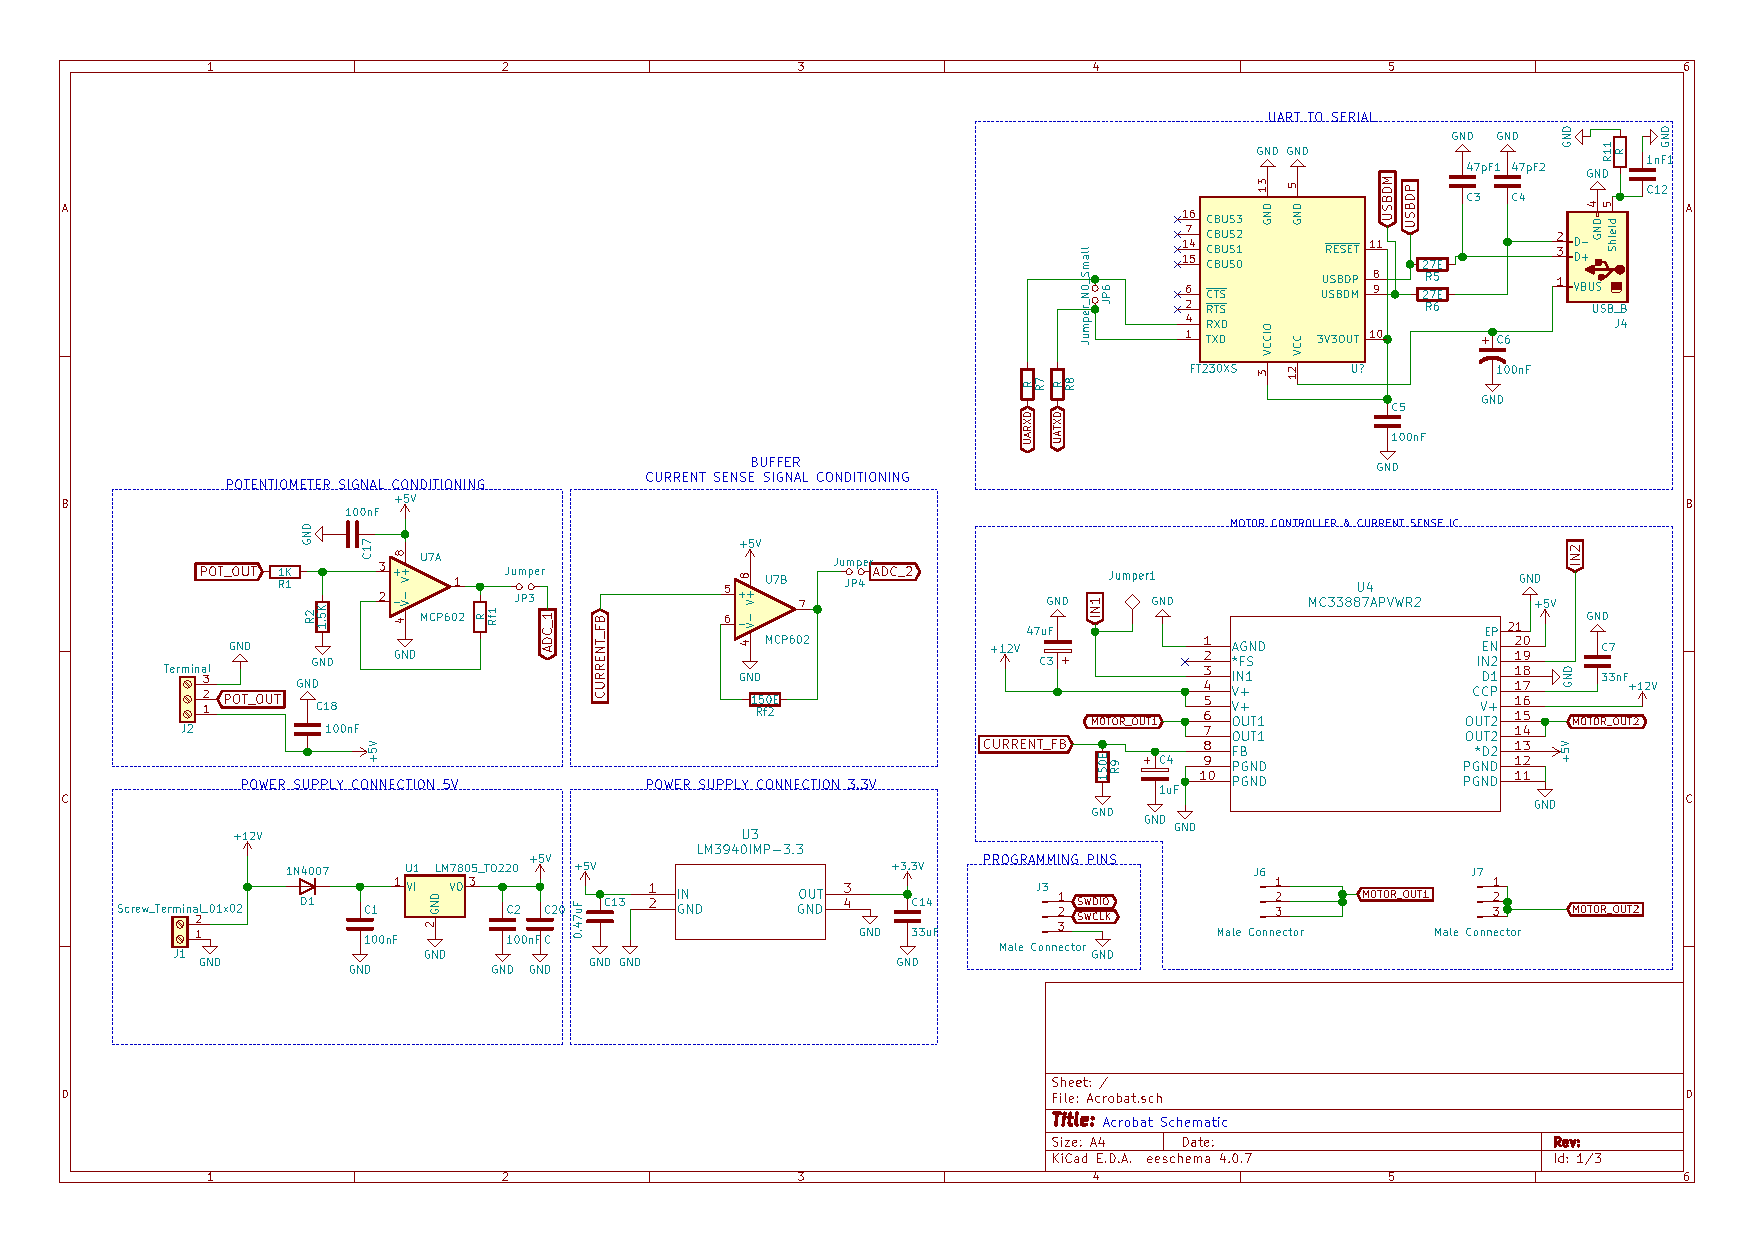
\includepdf[pages=1,pagecommand={\section{Electronic Design Schematic} \thispagestyle{empty} \label{sec:schematics}}, fitpaper=true]{./figs/Acrobat.pdf}
\includepdf[pages=2-,pagecommand={\thispagestyle{empty}}, fitpaper=true]{./figs/Acrobat.pdf}


\section{Communication Structure}
\label{sec:software_requirements}
\begin{figure}[h]
	\centering
	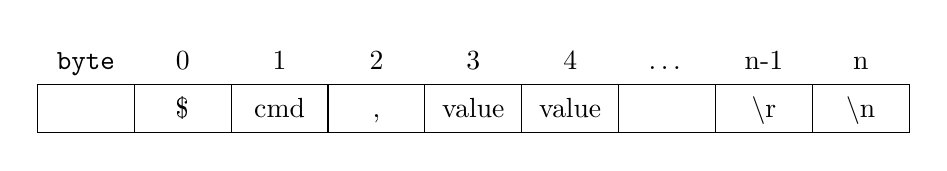
\begin{tikzpicture}[cell/.style={rectangle,draw=black},
	space/.style={minimum height=1.5em,matrix of nodes,row sep=-\pgflinewidth,column sep=-\pgflinewidth,column 1/.style={font=\ttfamily}},text depth=0.5ex,text height=2ex,nodes in empty cells]
	

	
	\matrix (first)[space, row 2/.style={minimum width=3em,nodes={cell,minimum width=3.5em}},row 3/.style={nodes={cell,minimum width=2em}}]
	{
		byte &0   & 1  & 2 & 3 & 4& \ldots & n-1&n  \\   
		&\$  & cmd  & , & value & value &  & \textbackslash r &  \textbackslash n \\};
	
	
	
	
\end{tikzpicture}
	\caption{Data Structure for Sending Commands}
	\label{fig:uart_struct_app}
\end{figure}

In Table \ref{table:uart_commands} the various commmands that are used in the command structure shown in Figure \ref{fig:uart_struct_app} used for debugging purposes is explained with the possible value ranges that can be used.


\begin{table}[h]
	\centering
	\begin{tabular}{|c|c|c|c|}
		\hline
		Command & Range &  Reason for Implementation & Effect \\
		\hline
		\hline
		A & None & Testing of the UART circuit & Send the following text: Feedback Control Of Robotic Gymnast\\
		\hline
		B & 0-100 &  & Changes PWM Duty-Cycle \\
		\hline
		C & 0-1 & Testing of AND digital Circuit Directional Control of Motor & Change the rotational direction \\
		\hline
		D & & & \\
		\hline
	
	\end{tabular}
	\caption{Summary of Communication Commands and their Effects}
	\label{table:uart_commands}

\end{table}


\newpage


%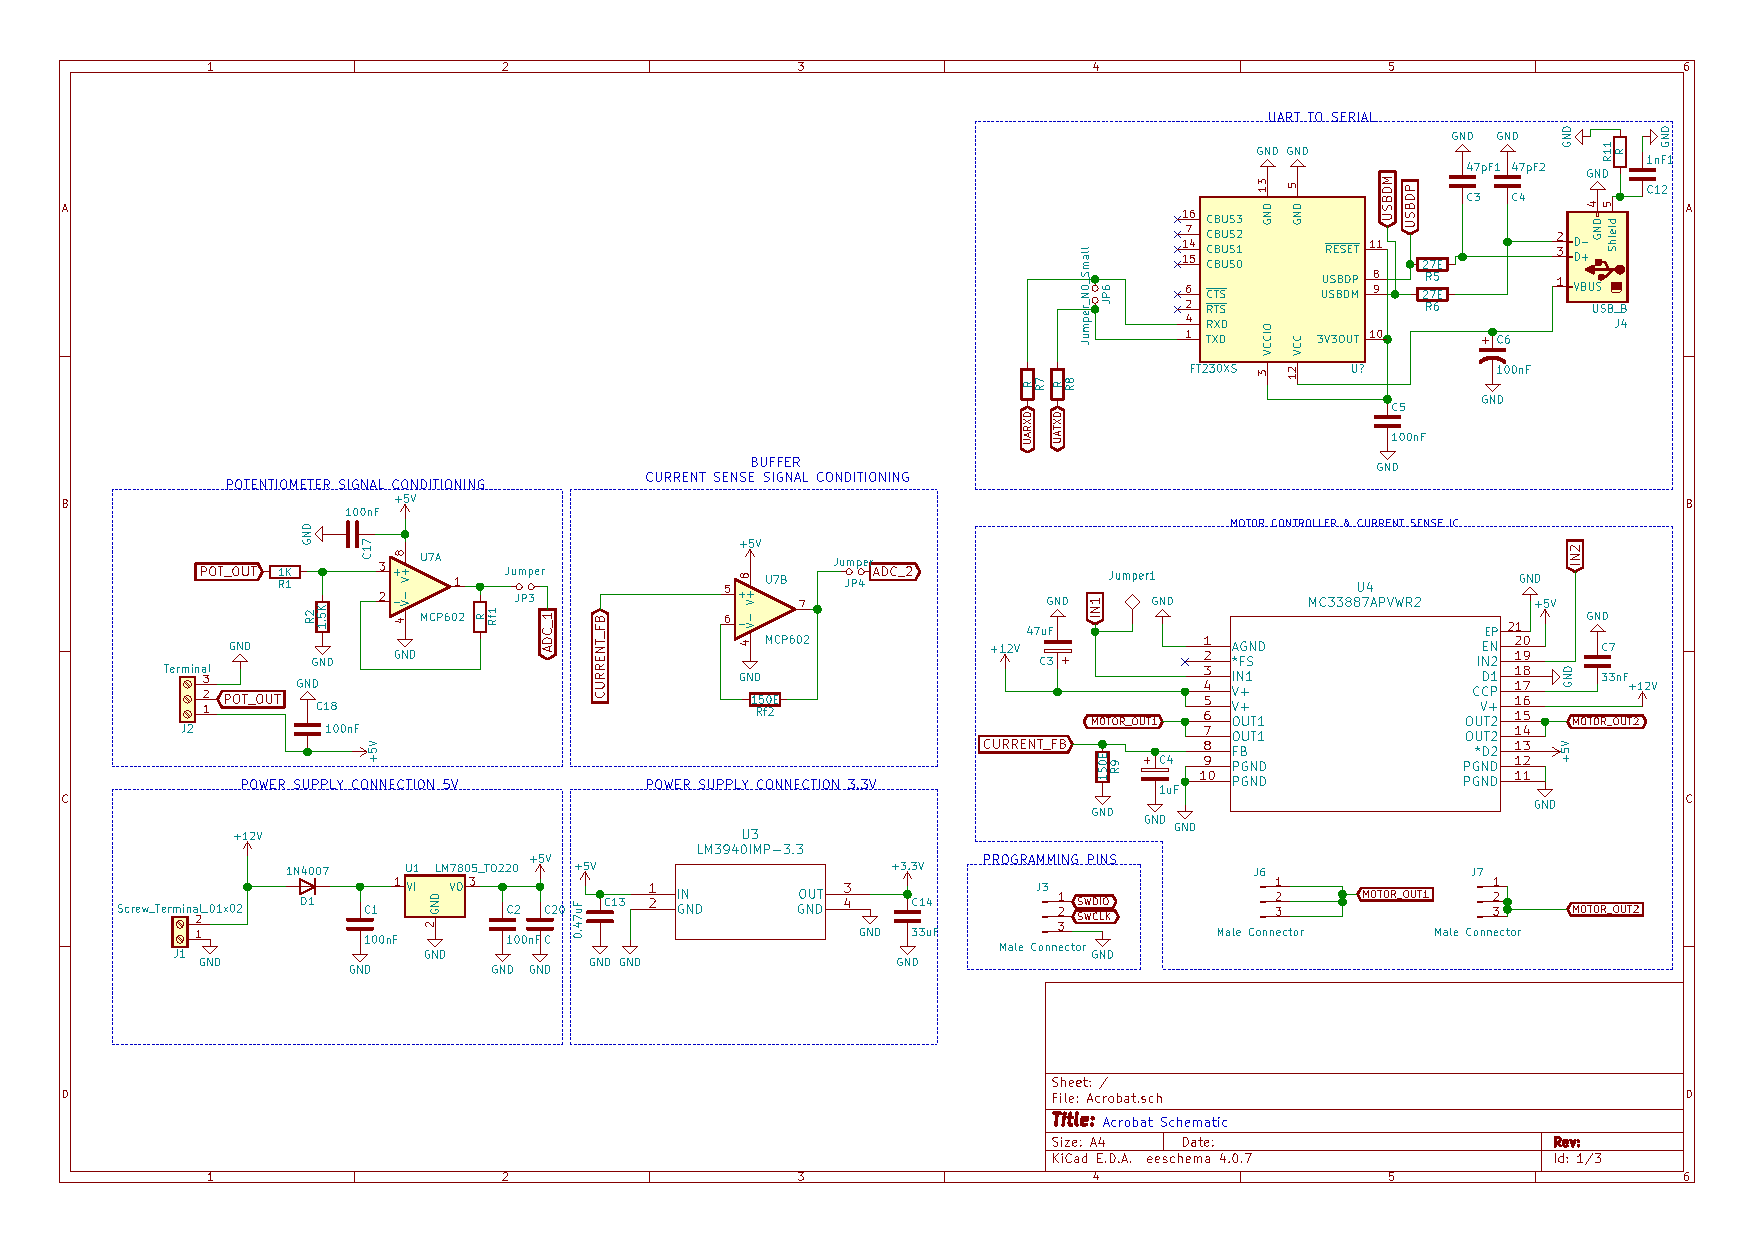
\includepdf[pages=-,scale-=0.8]{./figs/Acrobat.pdf}
%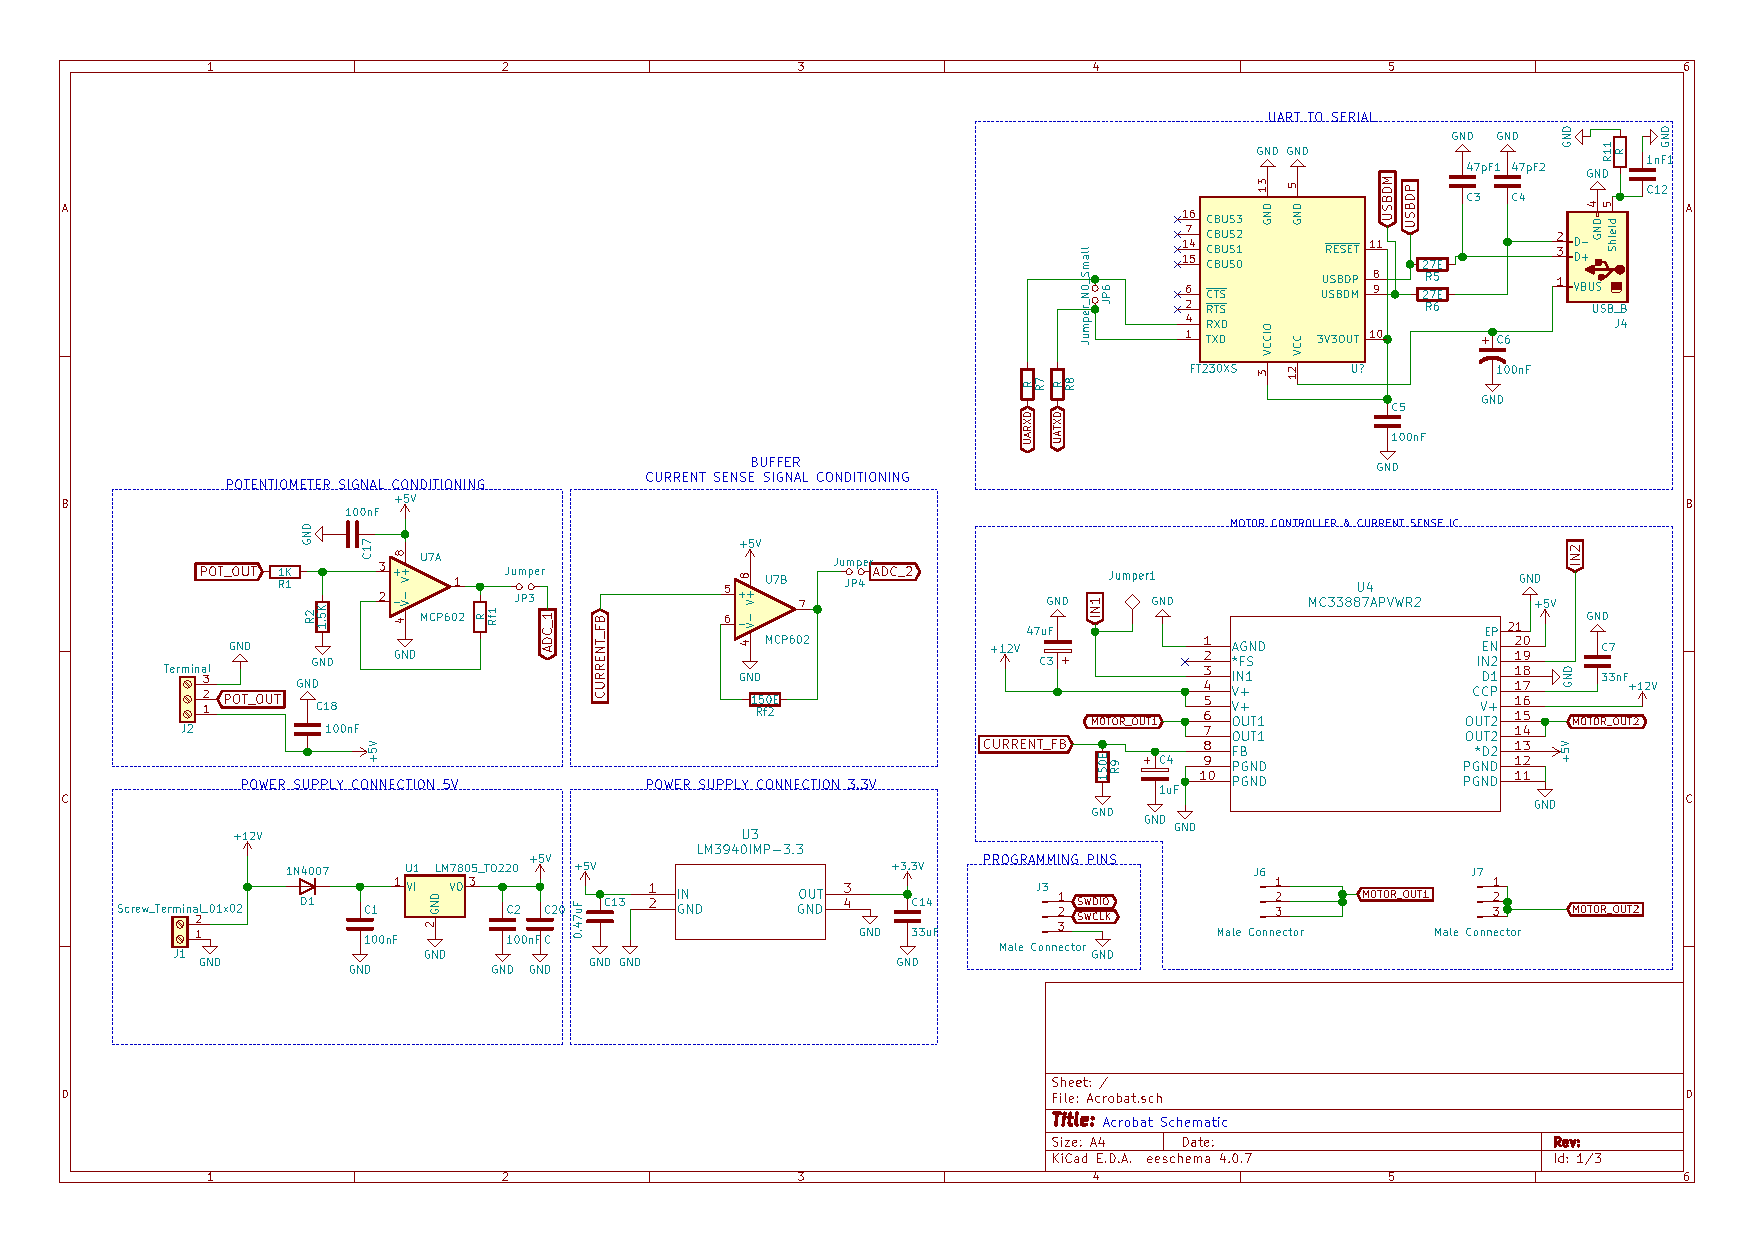
\includegraphics{./figs/Acrobat.pdf}





\section{Techno-Economy Assessment}
\label{sec:techno_eco}

\subsection{Budget}
The comparison between the proposed and actual budget is discussed and why the project was under-budget.\\

The proposed budget for the project was R3000. This budget was required to cover manufacturing cost and the buying of sensors, equipment and components. Table \ref{table:budget} provides the categories and amount of what the project consisted out of.\\

\begin{table}[h]
	\centering
	\begin{tabular}{|c|c|}
		\hline
		Category & Cost \\
		\hline
		\hline
		Electronic Components & R100 \\
		\hline
		Mechanical Components & R300 \\
		\hline 
		Software & R0 \\
		\hline
		Mechanical Manufacturing & R0 \\
		\hline
		Electronical Manufacturing & R0 \\
		\hline
		\hline 
		Total & R200 \\
		\hline
		
	\end{tabular}
	\caption{Categories of the Budget }
	\label{table:budget}
	
\end{table}

It is visible from the budget that the project is under-budget. The reason for being under-budget is due the Electrical and Electronic (E\&E) Deparment providing the service and components which were most expensive. This includes the manufacturing cost of the mechanical and electronic design and the Mechanical and Mechatronic Department providing the most expensive mechanical component.


\subsection{Planning}

\begin{figure}[h]
	\centering
	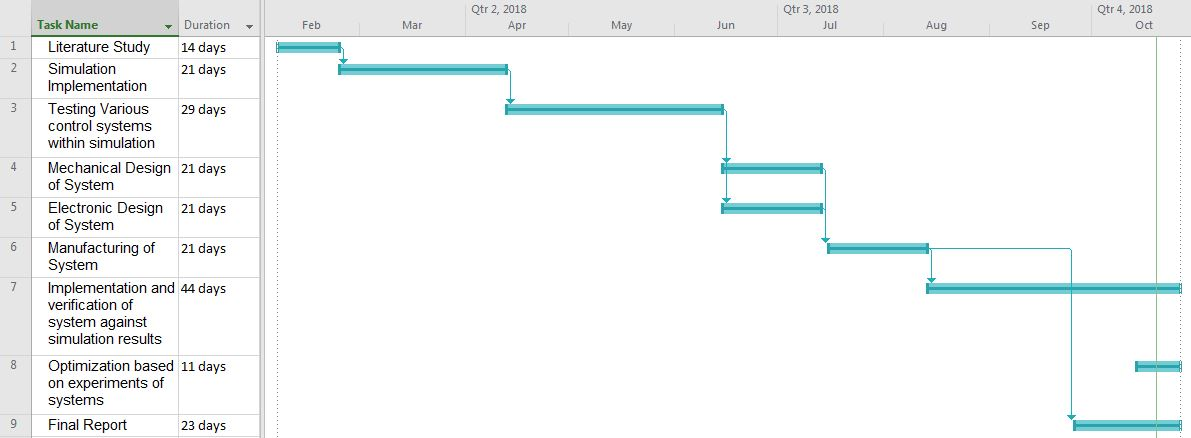
\includegraphics[scale=0.5]{./figs/planning_gantt/ganttchart.jpg}
	\caption{Planned Gantt Chart of the Project}
	\label{fig:planned_ganttchart}
\end{figure}

\begin{figure}[h]
	\centering
	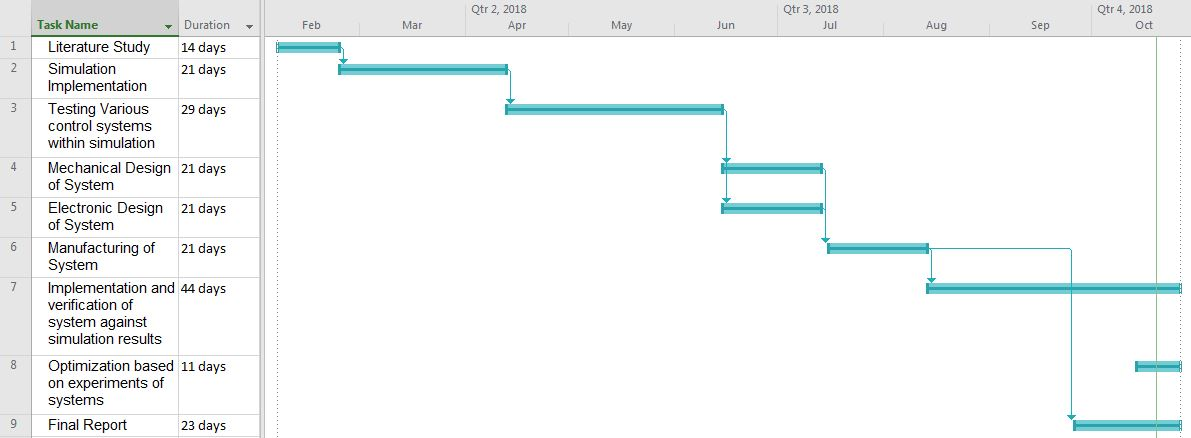
\includegraphics[scale=0.5]{./figs/planning_gantt/ganttchart.jpg}
	\caption{Actual Gantt Chart of the Project}
	\label{fig:actual_ganttchart}
\end{figure}

\begin{table}[h]
	\centering
	\begin{tabular}{|c|c|c|}
		\hline
		Category & Planned Hours & Actual Hours \\
		\hline
		\hline
		Simulation Implementation & 2 & 2 \\
		\hline
		Testing \& Verification of Simulation & 2 & 2 \\
		\hline 
		Mechanical Design  & 2 & 2 \\
		\hline
		Electronic Design & 2 & 2 \\
		\hline
		System Identification Test & 2 & 2 \\
		\hline
		Experiments & 2 & \\
		\hline
		Writing of Report & 2 & 2 \\
		\hline
		
	\end{tabular}
	\caption{Hours worked during the different phases of the project}
	\label{table:hours_worked}
	
\end{table}

Figure \ref{fig:planned_ganttchart} shows the Gantt chart for the planned activities during the project. For the majority of the project, the planned activities were followed as planned. All the activities from the literature study up to the implementation and verification of system results to simulation results.\\

During the experimental phase changes were required to the mechanical design which included a better connection between the motor shaft and actuated pendulum resulting in additional time required for the experiments. This additional time increased the safety during experiments and allowed the practical results presented in the report. This additional time was justified by using the time waiting for the part to be manufacture to write on my report.\\	

The electronic design took longer than what was planned due to experiencing difficulty programming the theoretical controllers on the microcontroller. It was decided to extend the time required for this phase due to without the controllers no practical results of these controllers would be acquired. It was decided to take an additional week to implement the controllers.\\

\subsection{Technical Impact}
The impact of the results presented in this report on the field of control systems, society and industry are discussed and whether the financial input was worthwhile.\\

The problem of the swinging and balancing of the robotic gymnast is a well research problem. Solutions to the swinging and balancing are provided on a theoretical level and supported by simulation results however little practical results are available of these theoretical solutions. The impact of this report includes the practical results of one of these theoretical implementation and discuss how the practical results differ from the theoretical results.\\

The impact of the practical results of this report on the industry of underactuated robotics are little. The robotic gymnast is a interesting problem and consist out of a highly non-linear and linear behaviour and is rather consider a great introductory problem to the field of underactuated robotics.\\

The impact of this report has little impact on society due to being of little interest on industry. The industry will not use the results and discussion presented in this report due to the reasons mentioned in the previous paragraph.\\

The financial input was worthwhile due to providing practical results on one theoretical implementation to the swinging and balancing of the robotic gymnast. \\


\subsection{Return on Investment}
The short and long term value from a technical and economical perspective is provided in this section. A motivation on the continuing research in the field of underactuated robotics are given and the financial cost to further research in this field.\\

Researching underactuated robotics is a exciting and growing research field due to the field of underactuated robotics have increasingly become more important due to technology growing in areas where control is crucial. Areas include: air drones, underwater inspection vehicles, space exploration and the aeroplane industry. \\

Underactuated robotics is an interesting and open field in control, with many design options to approach these types of problems. The most interesting examples of underactuated control problems are legged, swimming and flying robots that has been mentioned in the previous paragraph. This results in underactuated robotics being relevant in many fields.\\

The economical value of underactuated robotics in the short term and long term is high. Products are being brought to market that solve very difficult problems and can be used a broad variety. These products include \textit{Spot} from \textit{Boston Dynamics} which can be used for inspection, transportation and entertainment.\\

The financial cost to further the research on underactuated robotics are low due to the use of simulation programs that allows the testing of solutions on realistic simulated models. This significantly reduce the number of prototypes required to test the solution practically. 

\subsection{Potential for Commercialisation}\
The potential for the commercialisation of the contents within the report is discussed and the value of this commercialisations is given.\\

The contents does not have any real value for commercialisation. As mentioned earlier the problem researched is a very good introductory to underactuated robotics due to containing techniques that is a foundation for more advanced problems. 

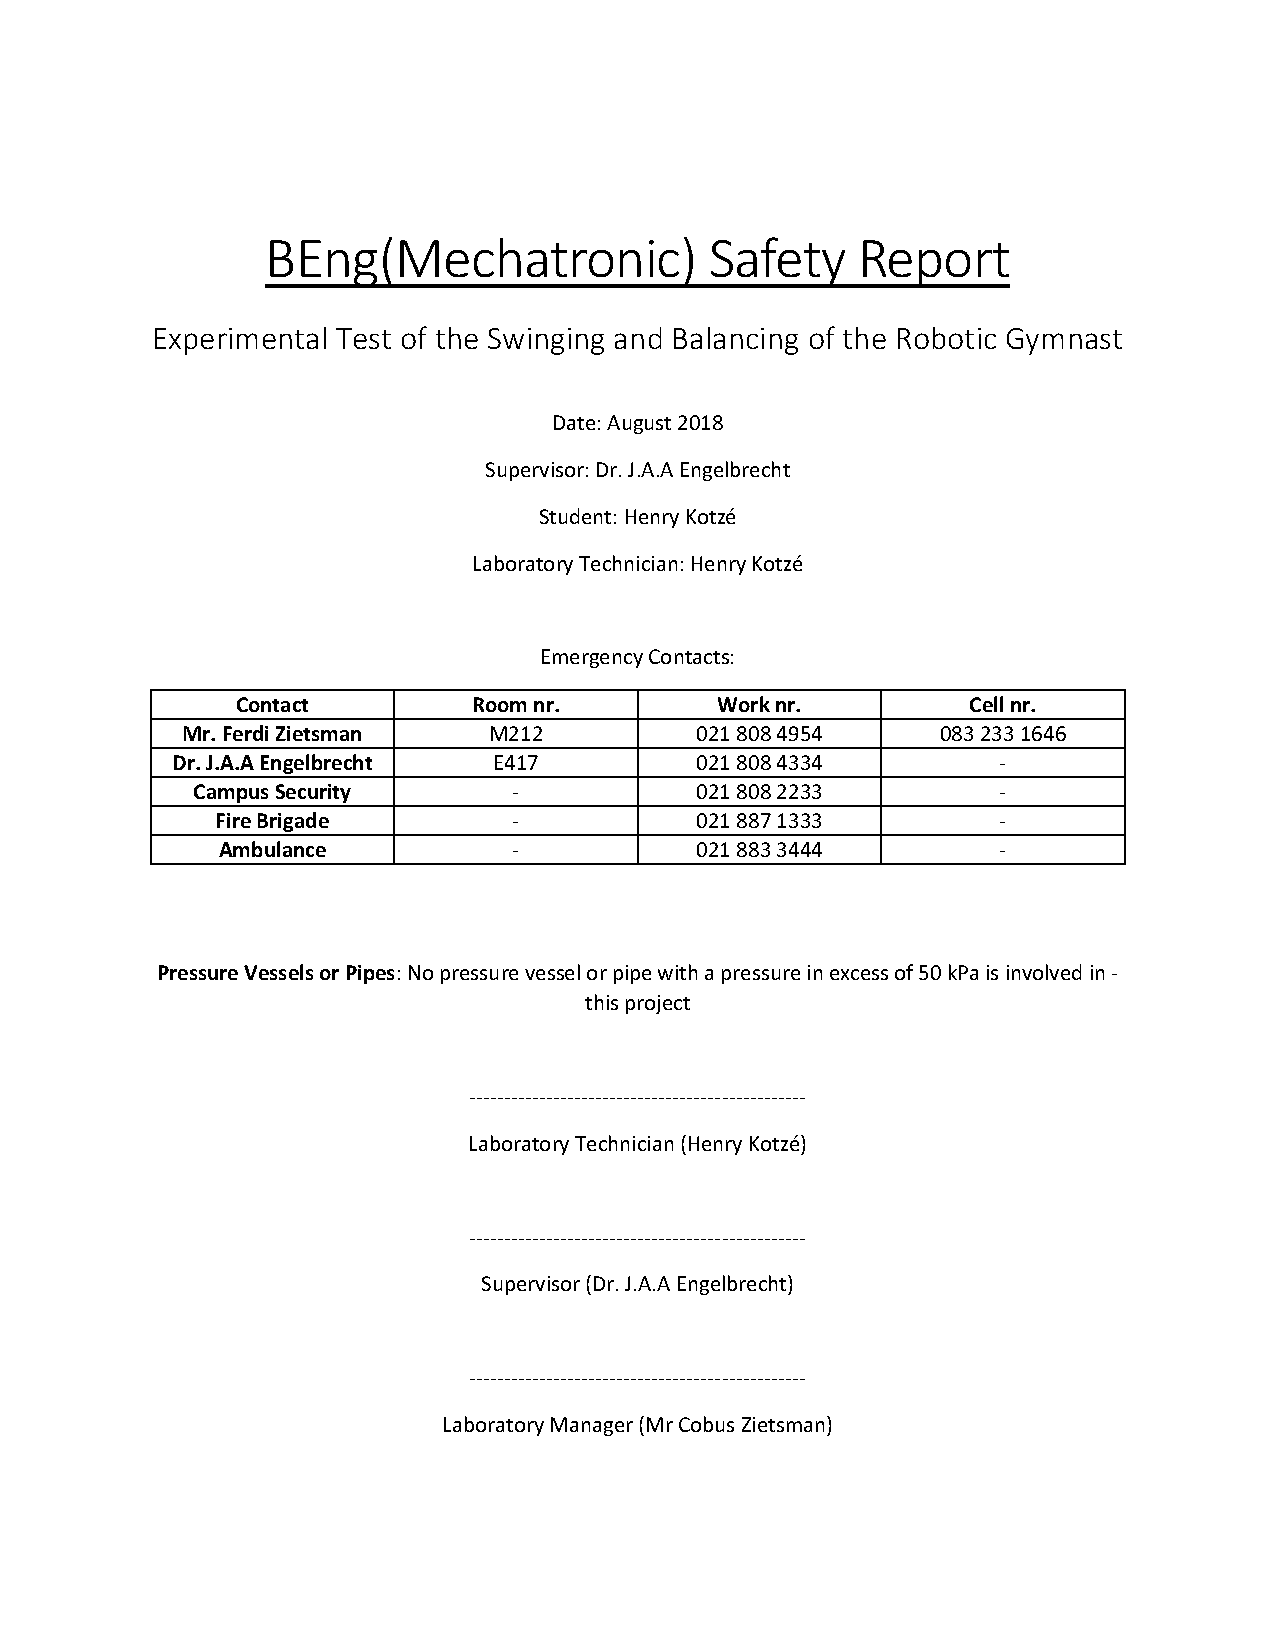
\includepdf[pages=1,pagecommand={\section{Risk Analysis \& Safety Procedures} \thispagestyle{empty} \label{sec:mech_drawings}}, fitpaper=true]{./figs/safety_report/safety_report.pdf}
\includepdf[pages=2-,pagecommand={\thispagestyle{empty}}, fitpaper=true]{./figs/safety_report/safety_report.pdf}

%----------------------------------------------------------------------------
\endinput

%\chapter{Feedback Control Design}
\label{chp:control}


\subsection{Feedback Linearisation}
\label{sec:colocated_linearisation}
%\include{contents/App-3}

%==== Bibliography acro's & Index ===================================
\backmatter

%\bibliography{backmatter/USbib-sample}

\end{document}
